% Figure 1: Correlations summary
\begin{figure}[htbp]
\centering
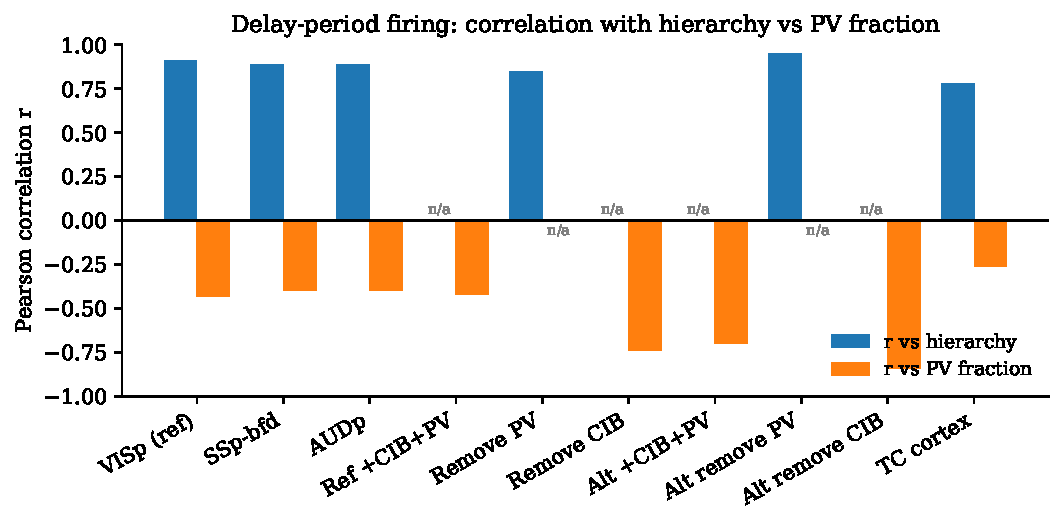
\includegraphics[width=0.98\textwidth]{figures/fig_corr_summary.pdf}
\caption{Pearson correlation of delay-period firing rate with cortical hierarchy and with PV cell fraction across the model scenarios reported in the experimental log. The visual (VISp), somatosensory (SSp-bfd) and auditory (AUDp) input conditions all yield $r\!\approx\!0.89$--$0.91$ with hierarchy and $r\!\approx\!-0.40$ to $-0.43$ with PV fraction. Control manipulations in the reference and alternative parameter regimes dissociate the contributions of the PV gradient and of counterstream inhibitory bias (CIB). ``n/a'' marks scenarios for which a value was not reported.}
\label{fig:corr_summary}
\end{figure}

% Figure 2: Graph-theoretic predictors
\begin{figure}[htbp]
\centering
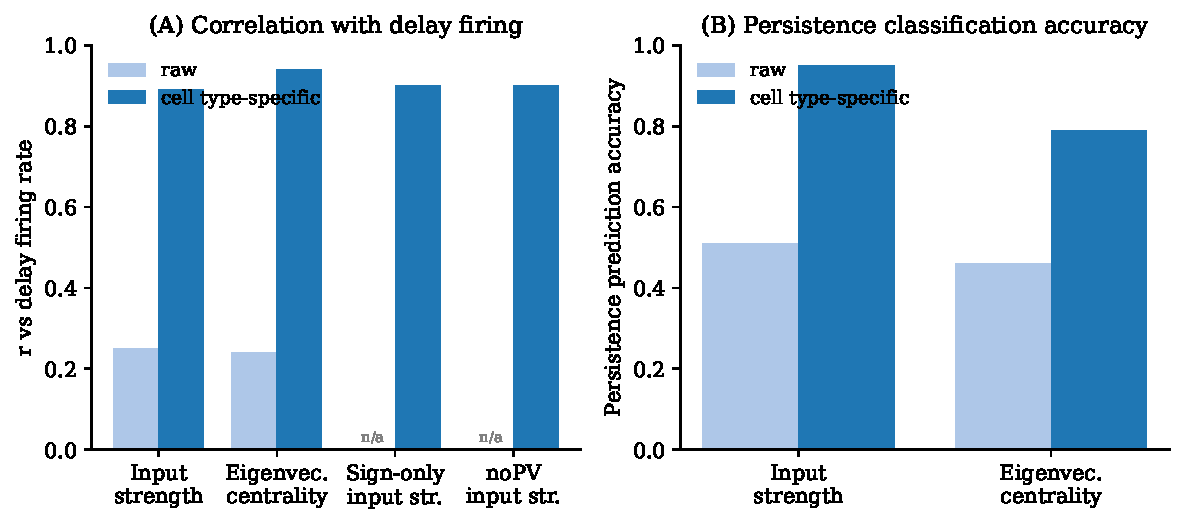
\includegraphics[width=0.98\textwidth]{figures/fig_measures.pdf}
\caption{Cell type-specific connectome measures predict delay firing where raw measures fail. (A) Raw input strength and raw eigenvector centrality are at best weakly correlated with delay firing rate ($r\!=\!0.25$ and $r\!=\!0.24$, respectively), whereas their cell type-specific counterparts reach $r\!=\!0.89$ and $r\!=\!0.94$. Sign-only and noPV input strengths attain $r\!=\!0.90$ each. (B) Classification of areas as persistent or non-persistent from raw versus cell type-specific measures: cell type-specific input strength reaches 95\% accuracy compared with 51\% from raw input strength; cell type-specific eigenvector centrality reaches 79\% compared with 46\%.}
\label{fig:measures}
\end{figure}

% Figure 3: Inhibition-effect decrements
\begin{figure}[htbp]
\centering
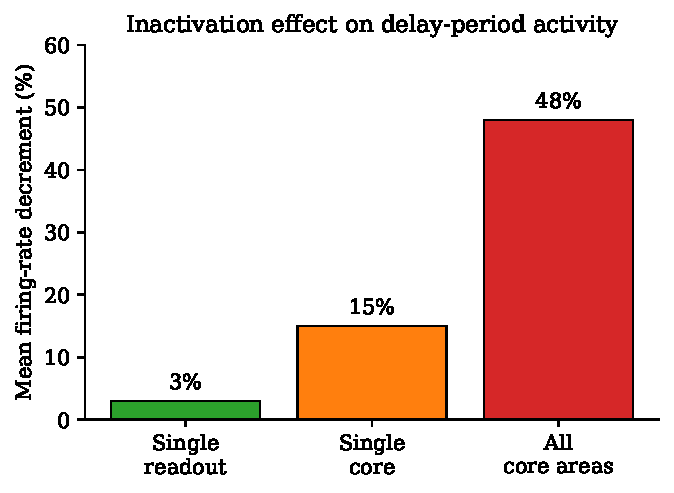
\includegraphics[width=0.55\textwidth]{figures/fig_inhibition.pdf}
\caption{Mean-firing-rate decrement of the areas that remain engaged in persistent activity, measured relative to the control simulation, after inactivation of different sets of cortical areas. Inhibition of a single readout area produces a 3\% decrement, inhibition of a single core area a 15\% decrement, and inhibition of all core areas simultaneously a 48\% decrement.}
\label{fig:inhibition}
\end{figure}

% Figure 4: Model schematic
\begin{figure}[htbp]
\centering

\includegraphics[width=0.9\textwidth]{figures/fig_model_schematic.pdf}
\caption{Schematic of the cell type-resolved multi-regional cortical model. Each of the 43 cortical areas is a mean-field circuit with two stimulus-selective excitatory pools ($E_1$, $E_2$) and a shared PV inhibitory pool whose strength scales with the area's PV cell fraction. Long-range projections from the Allen mesoscopic connectome are modulated by a hierarchy-dependent counterstream inhibitory bias: feedforward projections are biased toward excitatory cells in the target, feedback projections toward inhibitory cells. An optional 40-area thalamus (not depicted) is coupled to the cortex through AMPA-only projections that follow the same bias rule.}
\label{fig:schematic}
\end{figure}
